% Testing template
\begin{frame}
	\centering
	\frametitle{Testing}

	\begin{block}{Testing Strategy}
		
	 Comparing the number of expected repositories with actual repositories (Unit testing to verify the correctness of our system )
			\begin{center}
			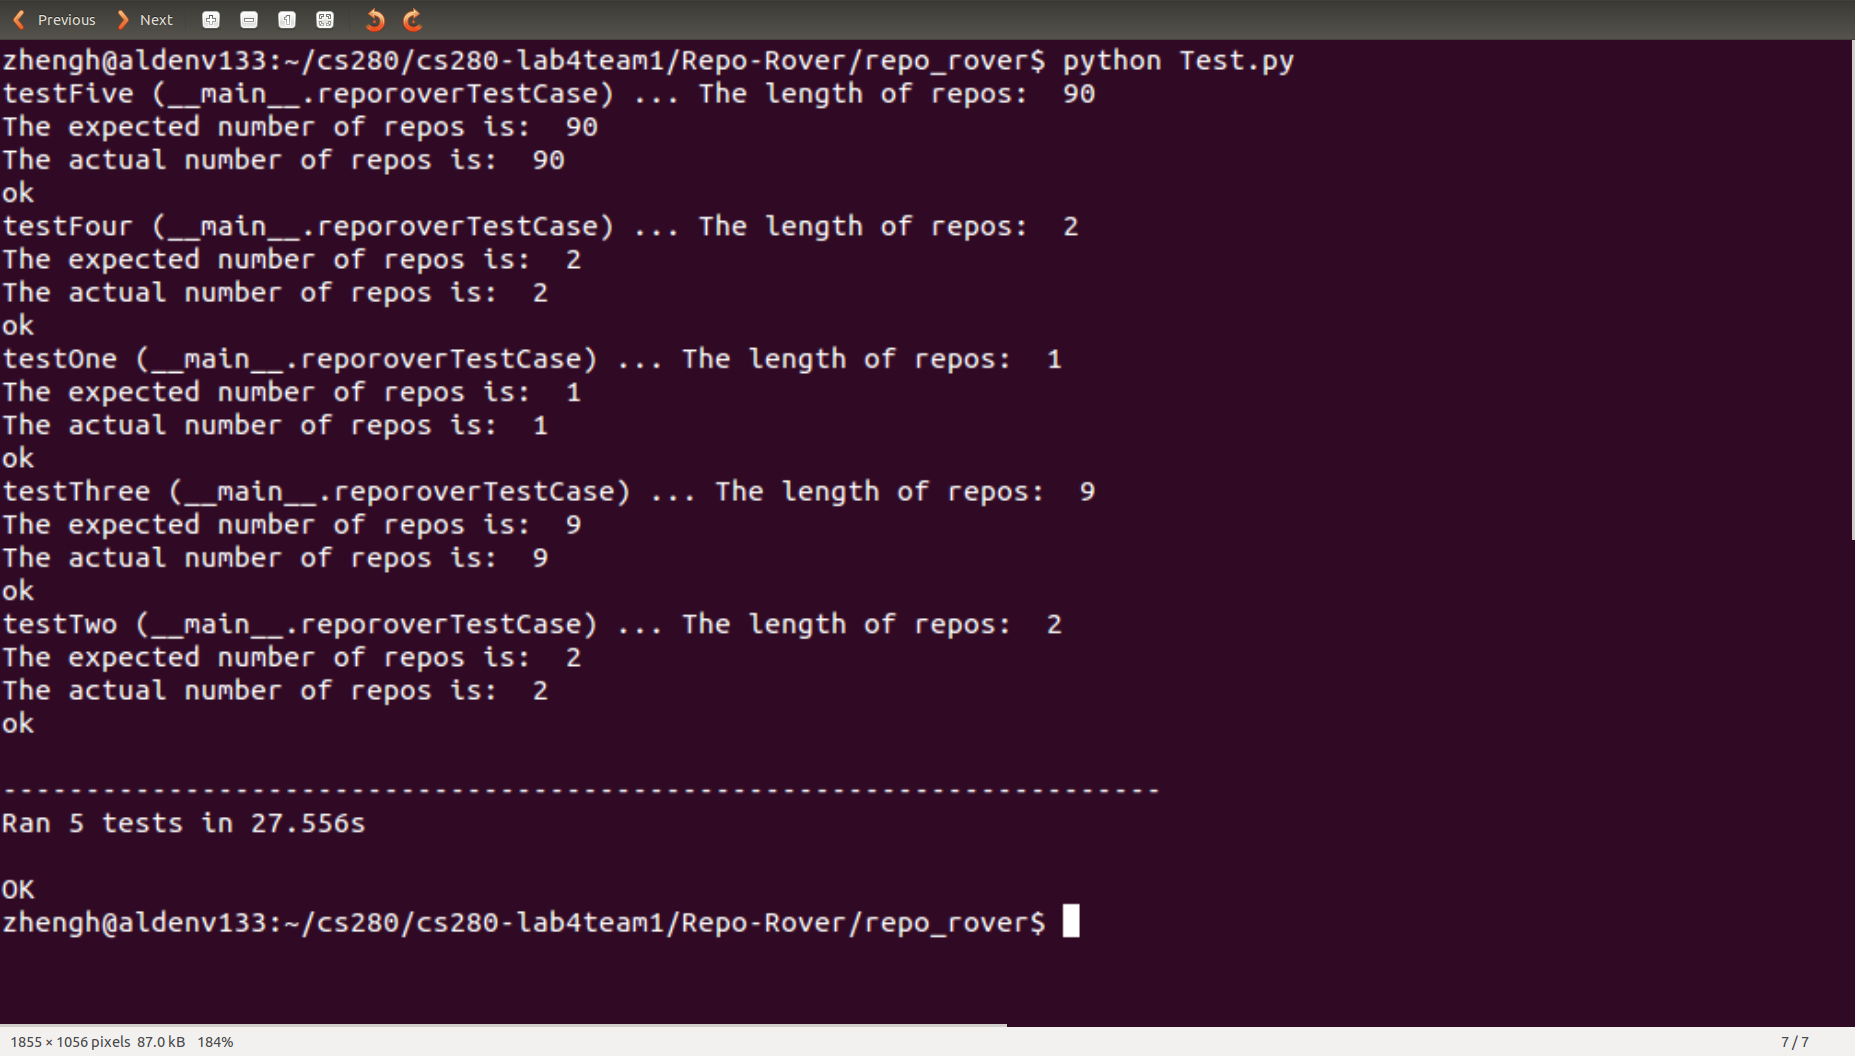
\includegraphics[width=10cm, height=5cm]{images/TestingResult.png}
			\end{center}
		
	\end{block}
	
\end{frame}

\begin{frame}
	\begin{block}{System Performance}
	The execution time of running the program with different repositories: 
		\begin{center}
			\begin{table}[]
			\centering
			\begin{tabular}{lll}
			\hline
 			1 Repository& 9 Repositories & 90 Repositories \\
 			0.217&1.285  &27.367    \\
 			\hline
 			0.218&1.275  &28.191    \\
 			\hline
 			0.203&1.281  &27.689		\\
 			\hline   
 			0.206& 1.279 & 27.514	\\
 			\hline
 			0.202& 1.283	 & 27.212	\\
 			\hline
 			Mean Value: & Mean Value: & Mean Value: \\
 			0.2092 & 1.2806	& 27.5946 
			\end{tabular}
			\end{table}
		\end{center}		
	\end{block}	
\end{frame}

\begin{frame}
	\begin{block}{System Performance}
	\begin{center}
	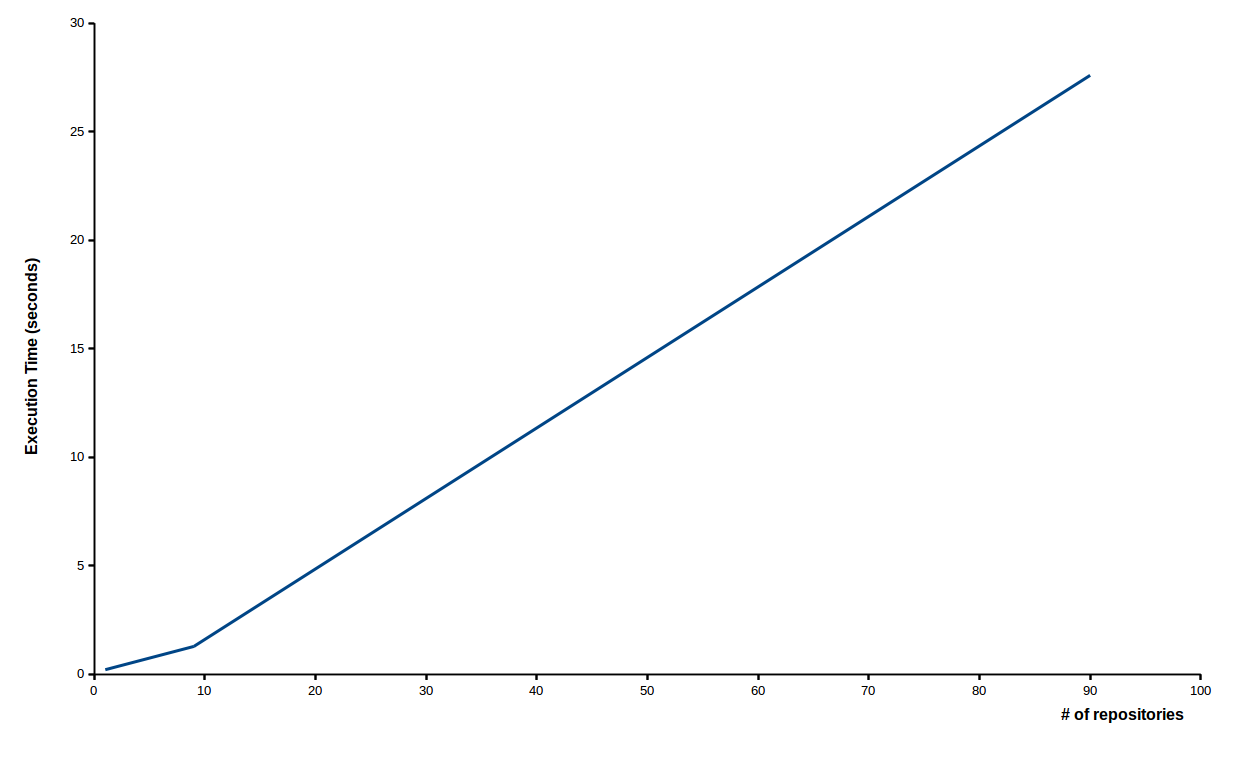
\includegraphics[width=10cm, height=7cm]{images/Execution.png}
	\end{center}
	\end{block}	
\end{frame}
